%FOR PDFLATEX USE ONLY
\documentclass[a4paper,12pt]{article}

\usepackage{amssymb,amsmath} %math symbols

\usepackage[margin=2cm]{geometry} %paper geometry

\usepackage[utf8]{inputenc} %allows unicode (including russian) source file
\usepackage[russian]{babel} %docment in russian-style
\usepackage[utf8]{inputenc}
%\usepackage[unicode]{hyperref} %links inside of the text
\usepackage[pdftex]{graphicx} %includegraphics pictures
\usepackage{cmlgc} %bold text

\usepackage{array} %arrays

%\usepackage{wrapfig}
%\usepackage{array}
%\usepackage{lipsum}
%\usepackage{esvect}
%\usepackage{hyperref}

\usepackage{subfig}
%\usepackage{calc}
%\usepackage{pgfplots,tikz,circuitikz}
%\usepackage{tkz-euclide}

\begin{document}

\begin{center}
  \LARGE{Работа 3.1.3}\\[0.2cm]
  \LARGE{Измерение магнитного поля Земли}\\[0.2cm]
  \large{Стрижак Даниил}\\[0.2cm]
\end{center}  
  

\section{Аннотация}

В работе исследуются свойства постоянных неодимовых магнитов и с их помощью находится горизонтальная и вертикальная составляющие индукции магнитного поля Земли, а так же магнитное наклонение.

\section{Теоретические сведения}

Простейший магнитный диполь может быть образован витком с током или постоянным магнитом. По определению, магнитный момент $m$ тонкого витка площадью $S$ с током $I$ равен $\mathfrak{m} = \frac{I\textbf{S}}{c}, $где $\textbf{S} = S\textbf{n}$ - вектор площади контура, образующий с направлением тока правовинтовую систему, $\textbf{n}$ - единичный вектор нормали к площадке. Если размеры контура с током или магнитной стрелки малы по сравнению с расстоянием до диполя, то соответствующий магнитный диполь называют \textit{элементарным}, или \textit{точечным}.

Магнитное поле точечного диполя определяется по формуле, анологичной формуле для поля элементарного электрического диполя:

\[ \textbf{B}_{дип} = \frac{3(\mathfrak{m} \cdot \textbf{r})}{r^5} - \frac{\textbf{m}}{r^3}\]

Во внешнем магнитном поле с индукцией $\textbf{B}$ на точеный магнитный диполь $\mathfrak{m}$ действует механический момент сил $\textbf{M}=[\mathfrak{m}, \textbf{B}] $
При этом потенциальная энергия которой обладает диполь с постоянным $\mathfrak{m}$, равна 
$W = -(\mathfrak{m} \cdot \textbf{B})$
Когда диполь ориентирован вдоль внешнего поля, он находится в состоянии \textit{равновесия}.

В \textit{неоднородном} внешнем поле выражение для энергии постоянного диполя сохраняется. При этом кроме момента сил на диполь действует ещё и сила 

\[\textbf{F} = -\nabla W = (\mathfrak{m} \cdot \nabla)\textbf{B}\]

Таким образом из вышесказанного следует, что \textit{свободный} магнитный диполь в неоднородном магнитном поле ориентируется вдоль силовых линий магнитного поля и втягивается в область более сильного поля, поскольку это ведёт к уменьшению энергии диполя.

Выражения выше, позволяют рассчитать силу взаимодействия магнитов с моментами $\mathfrak{m_1}$ и $\mathfrak{m_2}$. Kогда моменты двух небольших магнитов направлены вдоль соединяющей их прямой: $\mathfrak{m_{1,2}} \| \textbf{r}$, где $\textbf{r}$ - радиус-вектор между ними, они взаимодействуют с силой 
\[F_{12}= \mathfrak{m_1} \frac{\partial{B_2}}{\partial{r}} = \mathfrak{m_1}\frac{\partial{(2\mathfrak{m_2}/r^3)}}{\partial{r}} = -\frac{6 \mathfrak{m_1}\mathfrak{m_2}}{r^4} \;(ед.\; СГС) \]


Если магнитные моменты направлены перпендикулярно соединяющей их прямой: $\mathfrak{m_{1,2}} \perp \textbf{r}$, то нетрудно показать, что сила их взаимодействия окажется в два раза меньшей и будет иметь противоположный знак: $$F_{12} = \frac{3\mathfrak{m_1} \mathfrak{m_2}}{r^4}\;(ед.\; СГС).
 



\section{Оборудование и инструментальные погрешности}

\noindent \textbf{В работе используются:} неодимовые магниты; тонкая нить для изготовления крутильного маятника; медная проволока; электронные весы; секундомер; измеритель магнитной индукции; штангенциркуль; брусок, линейка и штатив из немагнитных материалов; набор гирь и разновесов.\\
\\
1.Весы -- 0.005 г \\
2.Секундомер -- 0.2 с \\
3.Штангенциркуль -- 0.01 см \\
4.Измеритель магнитной индукции -- 5\% ед. СГС \\


 \subsection{Экспериментальная установка}

В работе используются неодимовые магниты шарообразной формы. Важно, чтобы вещество из которого они изготовлены, было \textit{магнитожёстким} материалом и чтобы шары были намагничены однородно.

Магнитное поле однородного намагниченного шара радиусом $R$ может быть вычислено точно. На расстояниях $r \geq R$ от центра шара оно совпадает с полем \textit{точечного} магнитного диполя, расположенного в центре, магнитный момент $\mathfrak{m}$ которого совпадает с полным моментом шара. Внутри шара магнитное поле однородно. Hетрудно получить, что при $r < R$ \[\textbf{B}_{0} = \frac{2\mathfrak{m}}{R^3}\]

В качестве ещё одной характеристики материала магнита используют остаточную \textit{намагниченность} $\textbf{M}$. По определению, намагниченность равна \textit{объёмной плотности магнитного момента, поэтому для однородного намагниченного шара} $\mathfrak{m}= \textbf{M}V $, где $V = \frac{4\pi}{3}R^3$ - объём магнита. Величину $B_r = 4\pi \textbf{M}$ называют остаточной индукцией материала.

Из сказанного выше нетрудно видеть, что индукция $\textbf{B}_p$ \textit{на полсюсах} однородно намагниченного шара направлена по нормали к поверхности и совпадает поэтому с индукцией внутри шара $\textbf{B}_p = \textbf{B}_0$. Величина $B_p$ связана с остаточной индукцией $B_r$ соотношением \[B_p = B_o = \frac{2}{3}B_r \]

\section{Результаты измерений и обработка данных}
\subsection{Определение магнитного момента, намагниченности и остаточ- ной магнитной индукции вещества магнитных шариков}\\

Диаметр шариков измеряется с помощью штангенциркуля: $d = 0,585 \pm 0,005 $ см. \\
Масса шариков измеряется на весах, но для того, чтобы магнитное поле шариков не влияло на показания весов, сделаем толстую подложку из легкого материала -- бумаги. $m = 0,85 \pm 0,1 $ г. \\
Магнитометр показал значение $B_{p_1} = 380 \pm 5 (ед. \ СГС)$ на одном из полюсов, и значение $B_{p_2} = 330 \pm 5 (ед. \ СГС)$ на другом полюсе. 

\begin{center}
\begin{minipage}{0.4\textwidth}
 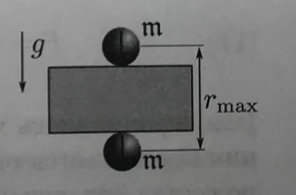
\includegraphics[width=\linewidth]{1.jpg}\\
Проложим между двумя магнитными шариками брусок из немагнитного материала как на рисунке сверху и, подкладывая между бруском и верхним магнитиком листы бумаги, определим, на каком максимальном расстоянии $r_{max}$ шарики удерживают друг друга в поле тяжести Земли. \[r_{max} = 2.18 \pm 0.05 \; {см}\]

Величина магнитного момента магнитика $\mathfrak{m}$:

\[ \mathfrak{m} = \sqrt{\frac{mgr^4_{max}}{6}} \]
\[ \mathfrak{m} = 71.3 \pm 3.4 \; (ед.\; СГС) \]

\end{minipage}
\begin{minipage}{0.05\textwidth}
\
\end{minipage}
\begin{minipage}{0.4\textwidth}
\begin{center}
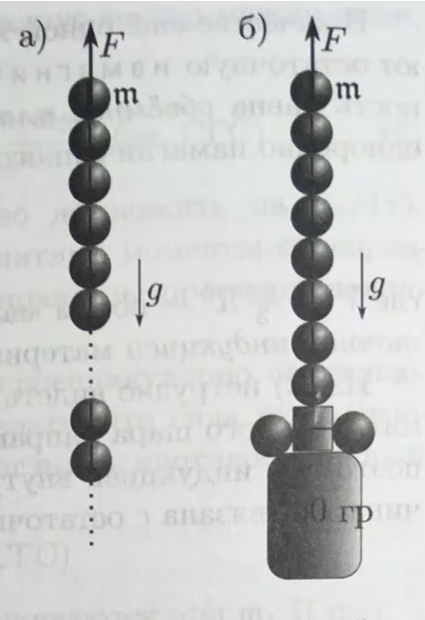
\includegraphics[width=0.7\linewidth]{2.jpg}\\
\end{center}
Составим цепочку из $25$ шариков, с помощью неодимовых магнитов в форме параллелепипедов, подсоединим цепочку к гире и разновесам так, чтобы общая масса системы составила приблизительно $500 \;г$. Далее подберём минимальный вес системы цепочки с гирей, при котором она отрывается от верхнего шарика.

Взвесим оторвавшуюся цепочку с гирей. $$m_{min} = 466.95 \pm 0.05 \; г$$

Рассчитаем силу сцепления двух шаров и по ней определим магнитный момент шарика $\mathfrak{m}$. 

\[ F_0 = \frac{6\mathfrak{m}^2}{d^4} \] \[F = m_{min}g  = F_0(1+\frac1{2^4}+\frac1{3^4} +...)\approx 1.08 F_0 \]

\[ \mathfrak{m} = \sqrt{\frac{d^4m_{min}g}{6 \cdot 1.08}} \;\]

\[\mathfrak{m} = 88.5 \pm 1.8 \; (ед. \; СГС).\]
\end{minipage}
\end{center}



Полученные значения магнитных моментов отличаются. Это может быть связано с большой погрешностью методики эксперимента, а так же неточным взаимным расположением магнитных моментов из-за силы трения. 

Величину намагниченности материала шариков рассчитаем по формуле $M = \frac{\mathfrak{m}}{\frac{\pi}{6} d^3}$, остаточную индукцию магнитного поля $B_r = \frac32B_0$. $$M = 875.1 \; (ед. \; СГС), \; B_r = 11000 \pm 550 \; (ед. \; СГС)$$

Табличное значение $B_r$ для соединения $Nd_2Fe_{14}B$:
$B_{r_{табл}} = 12200 \; (ед. \; СГС),$. Мы получили достаточно близкую величину к табличной. Из-за примесей и погрешности отличия допустимы. 

Теоретическое значение индукции $B_p$ у полюсов шарика c помощью формулы должно равняться:
$B_p = 7300 \; (ед. \; СГС)$, однако прибор показал значение на порядок меньше, что, вероятно связано с резким убыванием магнитного поля вблизи полюсов. 

\subsection{Горизонтальная составляющая магнитного поля Земли}

Оценим влияние упругости нити на период колебаний, возбудив крутильные колебания свёрнутой в кольцо "стрелки" (магнитный момент такого кольцеобразного маятника равен 0).

\begin{minipage}{0.3\textwidth}
Соберём крутильный маятник в виде кольца из 12 магнитных шариков и подвесим его на немагнитном штативе. Используя $\Lambda$- образный подвес, установим "магнитную стрелку" в горизонтальное положение, далее свернем её в кольцо и измерим коэффициент упругости нити

\end{minipage}
\begin{minipage}{0.05\textwidth}
\
\end{minipage}
\begin{minipage}{0.3\textwidth}
\begin{center}
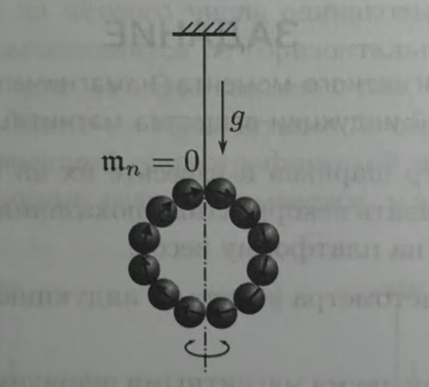
\includegraphics[width=\linewidth]{5.jpg}\\
\end{center}

\end{minipage}
\begin{minipage}{0.1\textwidth}
\
\end{minipage}
\begin{minipage}{0.3\textwidth}
\begin{tabular}{|c|c|c|}
		\hline
		N    & t, с  \\ 
		\hline
1   & 6.67 \\ 
		\hline
2     &13.34 \\ 
		\hline
 3     &  21.94 \\ 
		\hline
4     &  29.56\\ 
		\hline
 5     & 37.53 \\ 
		\hline
6     & 45.59 \\ 
		\hline
7     &  53.37\\ 
		\hline
8     & 61.11 \\ 
		\hline
9     &69.46 \\ 
		\hline
 10   & 77.32 \\ 
		\hline
	\end{tabular}

\end{minipage}
\\


\begin{center}
		\begin{tikzpicture}[scale = 1.0]
		\begin{axis}[
		axis lines = left,
		ylabel = {$T,c$},
		xlabel = {$n$},
		minor grid style={black, line width=0.05pt},
		major grid style={solid,black, line width=0.3pt},
		xmin=0, xmax=11,
		ymin=0, ymax=80,
		ymajorgrids = true,
		xmajorgrids = true,
		yminorgrids = true,
		xminorgrids = true,
		minor tick num = 4
		]
		\addplot+[only marks ] plot[error bars/.cd, y dir=both, y explicit]
		coordinates {
			(1,6.67)+-(0.3,0.3)
			(2,13.34) +-(0.3,0.3)
			(3, 21.94)+-(0.3,0.3)
			(4, 29.56)+-(0.3,0.3)
			(5, 37.53)+-(0.3,0.3)
			(6, 45.59)+-(0.3,0.3)
			(7, 53.37)+-(0.3,0.3)
			(8, 61.11)+-(0.3,0.3)
			(9, 69.46)+-(0.3,0.3)
			(10, 77.32)+-(0.3,0.3)
		};

		\addplot[blue, domain=0:20]{7.8*x-1};
		\end{axis}

		\end{tikzpicture}
		
\end{center}

\begin{center}
Зависимость времени колебаний от \\ числа колебаний кольца из магнитов. 
\end{center}

Из эксперимента получаем, что для кольца $T = 7.73 \; с$. Запишем уравнение вращательного движения и формулу для периода колебаний:
 
 $$I \ddot \alpha + f\alpha = 0, \; T = 2\pi \sqrt{\frac{I}{f}}, f = \Big(\frac{2\pi}{T}\Big)^2 I.$$
 Момент инерции относительно нити колечка можно оценить как $I = \frac{12mR^2}{2} = (2.5 \pm 0.1) \cdot 10^{-6} \; \frac{кг \cdot м^2}{c^2} \Rightarrow f =  (1.7 \pm 0.1) \cdot 10^{-6} \; \frac{кг \cdot м^2}{c^2}$. 
 
 \newpage

\begin{minipage}{0.45\textwidth}
Соберём крутильный маятник из 12 магнитных шариков и подвесим его на немагнитном штативе. Используя $\Lambda$- образный подвес, установим "магнитную стрелку" в горизонтальное положение.
Возбудим крутильные колебания маятника вокруг вертикальной оси и определим их период. Исследуем зависимость периода $T$ крутильных колебаний "стрелки" от количества магнитных шариков n, составляющих "стрелку". 
\end{minipage}
\begin{minipage}{0.1\textwidth}
\
\end{minipage}
\begin{minipage}{0.45\textwidth}
\begin{center}
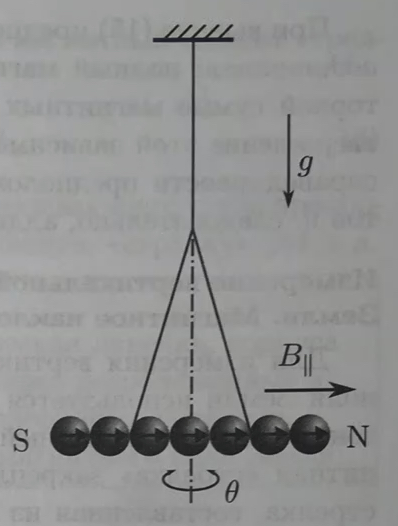
\includegraphics[width=0.7\linewidth]{3.jpg}\\
\end{center}
\end{minipage}

\\

	\begin{tabular}{|l|l|l|l|l|l|l|l|l|l|l|}
		\hline
		n	& 3     & 4     & 5     & 6     & 7     & 8     & 9      & 10    & 11    & 12    \\ \hline
		N    & t, с  & t, с  & t, с  & t, с  & t, с  & t, с  & t, с   & t, с  & t, с  & t, с  \\ \hline
		10   & 6.35  & 9.33  & 11.18 & 13.33 & 16.56 & 17.70 & 20.20  & 23.50 & 23.89 & 27.60  \\ \hline
		20   & 18.67 & 18.51 & 22.00 & 26.66 & 32.79 & 35.40 & 40.40  & 44.17 & 47.61 & 51.26 \\ \hline
		30   & 24.91 & 27.68 & 33.45 & 39.70 & 43.35 & 52.83 & 61.93  & 66.29 & 70.33 & 77.85 \\ \hline
		40   & 31.21 & 36.77 & 44.01 & 53.00 & 65.91 & 70.00 & 82.03  & 88.09 & 93.91 & 104.5 \\ \hline
		50   & 37.45 & 46.01 & 56.11 & 67.00 & 82.47 & 87.58 & 102.10 & 109.4 & 117.2 &130.3 \\ \hline
		T, c & 0.749 & 0.920 & 1.122 & 1.340 & 1.649 & 1.752 & 2.042  & 2.188 & 2.344 & 2.606 \\ \hline
	\end{tabular}
	
\\

График экспериментальной зависимости $T(n)$: \\
\begin{center}
\begin{tikzpicture}[scale = 1.0]
		\begin{axis}[
		axis lines = left,
		legend style={at={(1,0.133)}},
		ylabel = {$T,c$},
		xlabel = {$n$},
		minor grid style={black, line width=0.05pt},
		major grid style={solid,black, line width=0.3pt},
		xmin=2, xmax=12,
		ymin=0, ymax=3,
		ymajorgrids = true,
		xmajorgrids = true,
		yminorgrids = true,
		xminorgrids = true,
		minor tick num = 4
		]
		\addplot+[only marks ] plot[error bars/.cd,  y dir=both, y explicit]
		coordinates {
			(3,0.75)+-(0.1,0.1)
			(4,0.92) +-(0.1,0.1)
			(5, 1.12)+-(0.1,0.1)
			(6, 1.34)+-(0.1,0.1)
			(7, 1.65)+-(0.1,0.1)
			(8, 1.75)+-(0.1,0.1)
			(9, 2.04)+-(0.1,0.1)
			(10, 2.19)+-(0.1,0.1)
			(11, 2.34)+-(0.1,0.1)
			(12, 2.61)+-(0.1,0.1)
		};

		\addplot[blue, domain=0:20]{0.207*x + 0.115};
		\end{axis}
		\end{tikzpicture}
\end{center}

\begin{center}
Зависимость периода колебаний от \\ числа числа магнитов магнитной стрелки. 
\end{center}

 \[J_n \ddot\theta + (\mathfrak{m}_n B_{\|}+f)\theta = 0, J_n \approx \frac1{12}n^2md^2 \Rightarrow T_n = 2\pi \sqrt{ \frac{md^2n^2}{12(\mathfrak{m}B_{\|}+f)}}\]
По значению углового коэффициента рассчитаем величину горизонтальной составляющей магнитного поля Земли.
$$\frac{T_n}{n} = 2\pi \sqrt{ \frac{md^2n^2}{12(\mathfrak{m}B_{\|}+f)}} = 0.207 \; c, B_{\|} = \frac{\pi^2 md^2n^2}{3 T_n^2 \mathfrak{m}} - \frac f{\mathfrak {m}}\approx 0.066 \pm 0.003 \; (ед. \; СГС) $$

\newpage

\begin{minipage}{0.45\textwidth}

Изготовим магнитную "стрелку" из 10 шариков и подвесим её за середину с помощью нити на штативе.
Определим механический момент сил, действующий со стороны магнитного поля Земли на \textit{горизонтально} расположенную магнитную "стрелку". Для этого с помощью одного или нескольких кусочков проволоки, уравновесим "стрелку" в горизонтальном положении.
С помощью весов определим массу уравновешивающего груза $m_{гр}$.
Из условия равновесия рассчитаем механический момент сил $M = m_{гр}gx$, действующих на горизонтальную "стрелку"  со стороны поля Земли. Измерения сил проведём для чётных значений $n = 4,6,8,10,12$.
\end{minipage}
\begin{minipage}{0.05\textwidth}
\
\end{minipage}
\begin{minipage}{0.45\textwidth}
\begin{center}
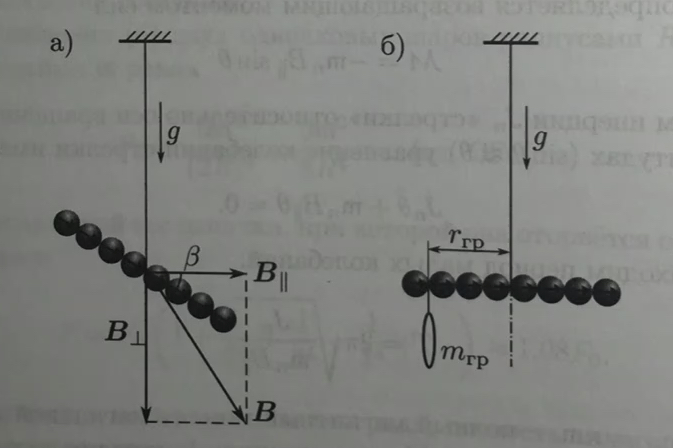
\includegraphics[width=\linewidth]{4.jpg}\\
\end{center}
\end{minipage} 

\\

\begin{center}
\begin{tabular}{|l|l|l|l|}
		\hline
		n  & $m_{гр}$, г  & x, см & M, $г\frac{см^2}{с^2}$ \\ 
		\hline
		4  & 0.215 & 0.585 & 123.4  \\ 
		\hline
		6  & 0.196 & 1.170 & 224.9   \\
		 \hline
		8  & 0.149 & 1.755 & 256.5   \\ 
		\hline
		10 & 0.154 & 2.340 & 354.6   \\ 
		\hline
		12 & 0.165 & 2.925 & 472.8   \\ 
		\hline
\end{tabular}
\end{center}

\begin{center}

		\begin{tikzpicture}[scale = 1.3]
		\begin{axis}[
		axis lines = left,
		legend style={at={(0.8,0.9)}},
		ylabel = {$M,\; г\frac{см^2}{с^2}$},
		xlabel = {$n$},
		minor grid style={black, line width=0.05pt},
		major grid style={solid,black, line width=0.3pt},
		xmin=2, xmax=13,
		ymin=100, ymax=500,
		ymajorgrids = true,
		xmajorgrids = true,
		yminorgrids = true,
		xminorgrids = true,
		minor tick num = 1
		]
		
		\addplot+[only marks ] plot[error bars/.cd, y dir=both, y explicit]
		coordinates {
			(4, 123.4) +-(15,15)
			(6, 224.9)+-(15,15)
			(8, 266.5)+-(15,15)
			(10, 354.6)+-(15,15)
			(12, 472.8)+-(15,15)
		};
		\addplot[blue, domain=0:20]{40*x - 27};		
		\end{axis}
		\end{tikzpicture}	

\end{center}

\begin{center}
Зависимость момента сил, уравновешивающего \\ стрелку от числа числа магнитов в ней. 
\end{center}

Коэффициент наклона $a = 36 \pm 5 \; г\frac{см^2}{с^2}.$ Из линейности видно, что приближение аддитивности магнитных моментов для используемых в работе магнитов применимо. По значению углового коэффициента аппроксимирующей прямой рассчитаем величину вертикальной составляющей $B_{\perp}$ магнитного поля Земли.
$$M_n = n\mathfrak{m}B_{\perp} \Rightarrow B_{\perp} = \frac{a}{\mathfrak{m}} \approx 0.40 \pm 0.06 \; (ед. \; СГС)$$



\newpage
\section{Выводы и рассчет погрешностей}
\subsection{Погрешности}

\[ \varepsilon_{\mathfrak{m_1}} = \sqrt{\Big(\frac{\Delta m}m\Big)^2 + 4\Big(\frac{\Delta r_{max}}{r_{max}}}\Big)^2} \approx 6 \%\]

\[ \varepsilon_{\mathfrak{m_2}} = \sqrt{\Big(\frac{\Delta d}d\Big)^2 + 4\Big(\frac{\Delta r_{min}}{r_{min}}}\Big)^2} \approx 2 \%\]

\[\varepsilon_{B_{\|}} = \sqrt{\Big(\frac{\Delta m}m\Big)^2 + \Big(\frac{\Delta d}d\Big)^2 + \Big(\frac{\Delta \mathfrak{m}}{\mathfrak{m}}\Big)^2 + \Big(\frac{\Delta \frac{T_n}{n}}{\frac{T_n}{n}}\Big)^2} \approx 5 \% \]

\[\varepsilon_{B_{\perp}} = \sqrt{(\Big(\frac{\Delta a}a\Big)^2 + \Big(\frac{\Delta \mathfrak{m}}{\mathfrak{m}}\Big)^2} \approx 6 \%\]


\subsection{Вывод}
Поскольку  установка находится в железобетонном
здании, магнитное поле в нём сильно отличается от поля Земли. Так же на
показания влияет наличие электронных приспособлений связи. Магнитное
поле Земли в нашем районе около 0.05 - 0.1 ед. СГС. Полученное значение не сильно отличается действительного.  

Используя результаты измерений $B_{\perp]}$ и $B_{\|}$, магнитное наклонение $\beta$ и полная величина индукции магнитного поля Земли в кабинете выполнения лабораторной работы равны. 
$$\beta = \arctan{\frac{B_{\perp}}{B_{\|}}} \approx 80^{\circ}  $$

Теоретически ($\alpha - угол\ наклона\ Земли,\ \phi - широта\ Москвы $), 
\[\beta = \frac{B_{\perp}}{B_{\|}} = \frac{\frac{-2\matfrac{m}_3sin(\phi-\alpha)}{r^3}}{\frac{-\matfrac{m}_3cos(\phi-\alpha)}{r^3}} = arctg(2 tg(\phi - \alpha)) \approx 53^{\circ}\].

Полный магнитный момент $\mathfrak{m_{з}}$ Земли равен около $7,72 \cdot 10^{25}$ ед.  СГС. По данным эксперимента он равен $9,20 \cdot 10^{25}$ ед. СГС. 


\end{document}
